\chapter{Introduction}

\todo{Preface}

This report serves as a Master's thesis in Applied Computer Science at \acrfull{ntnu} written in the spring semester of 2021. It explores topics surrounding vessel destination prediction for the purpose of maritime logistics. The author of the thesis has a prior Bachelor’s degree in Programming (Applications) from \acrshort{ntnu}, and the thesis was conducted in collaboration with the maritime technology startup company called \acrfull{mo} where the author is currently employed as a part-time developer.


\section{Topics covered by project}
\label{sec:topics_covered}

The topics covered by this project mainly include applying computer science techniques to the problem of predicting maritime vessel's future destinations and voyage patterns to aid different actors in the shipping industry in their daily decision-making processes. More specifically, the thesis focuses on the aspect of using \acrfull{ml} techniques with different sources of vessel information such as \acrfull{ais}, voyage patterns, and detailed information about specific vessels. The goal of the thesis is to establish a high-quality, general prediction method not restricted by geographical extent or specific time intervals, and to discuss possible applications and value of the model in the current state of the art of the shipping industry.

\section{Keywords}

AIS data, vessel destination prediction, vessel supply, machine learning, maritime logistics

\section{Problem description}
\label{sec:problem_desc}

The current methods used in the shipping industry normally require extensive manual labor to gather data for analysis. The industry is still prone to using non-digital methods and external services to provide relevant information about vessel supply and traveling patterns. Most actors in the industry heavily rely on predicting the market in order to make smart decisions resulting in beneficial investments. In order to predict the market the most important factors are cargo demand and vessel availability. % (\cref{fig:maritime_economics})

% \begin{figure}[htbp]  % order of priority: h here, t top, b bottom, p page
%     \centering
%     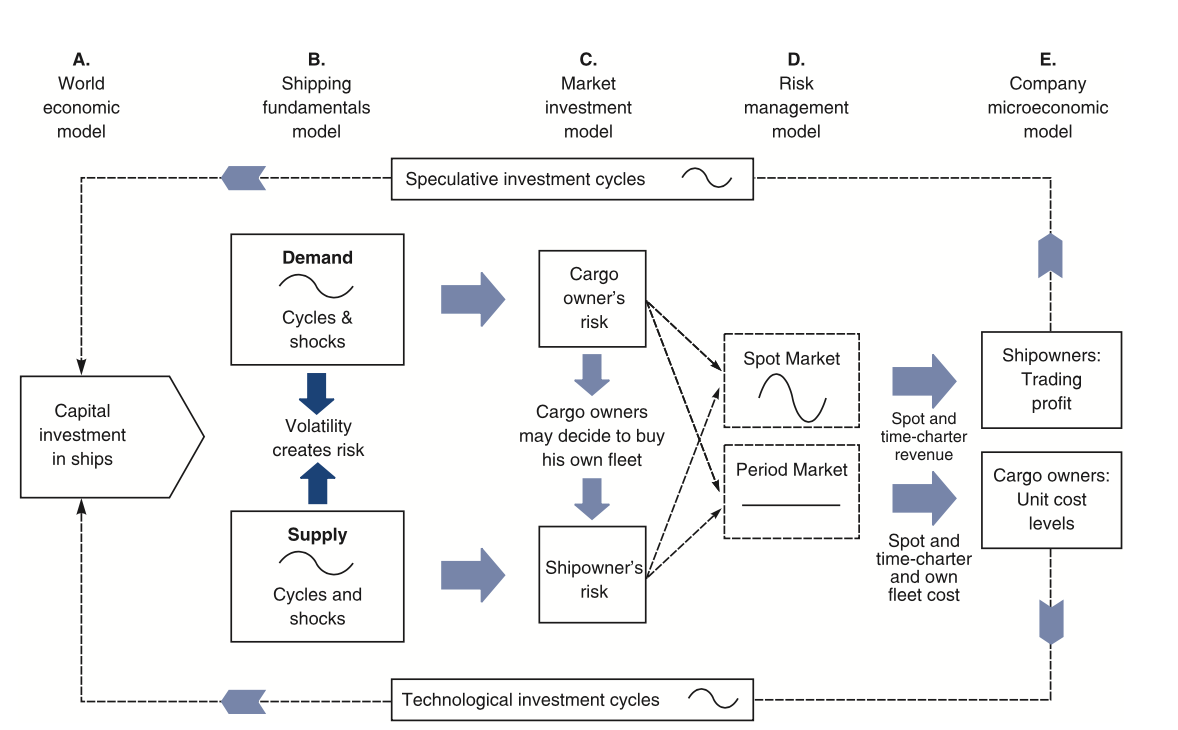
\includegraphics[width=.89\textwidth]{figures/investment_cycle}
%     \caption{Vessel supply’s impact on the market and investment cycles \parencite{stopford2008}}
%     \label{fig:maritime_economics}
% \end{figure}


Furthermore, the data used to make such predictions are generally considered proprietary in the industry which is hesitant to share information. However, in recent years, sources of vessel information have become more available through the \acrshort{ais} standard that provides information such as vessel positions, navigational statuses, and manually inputted voyage information. In 2004, the \acrfull{imo} initiated the \acrshort{ais} protocol which all commercial vessels over 299 \acrfull{gt} are required to use. This provides a plentiful source of information applicable toward analysis of vessel availability on a global scale.

Although the \acrshort{ais} protocol contains voyage information such as intended destination port and the estimated time of arrival (ETA), since this information is manually input by crew members, it is not standardized and often prone to human error in regards to either format or misinformation. \cite{mestl2016} claims the accuracy of this information to be as low as 4\% in certain areas. In order to use \acrshort{ais} data, existing prediction methods, therefore only consider the geographical information that is automated thus mostly accurate similar to that of GPS\@. On the other hand, other aspects such as vessel type, dimensions, and draft, have extensively been overlooked in such methods limiting them in terms of accuracy when applied to a general range of vessels. Therefore, this thesis proposes an approach that takes advantage of a broader range of vessel information in order to make more reliable vessel destination predictions.

\section{Justifications, motivation, and benefits}
\label{section:justifications_motivations_benefits}

The shipping industry is a vast industry that affects the entire world in some manner. It is generally believed to be responsible for \textit{90\%} of all world trade \parencite{grote2016} but is also a massive contributor to global air pollution which negatively affects the environment \parencite{zheng2016:online}. These factors leave room for innovation in terms of optimization as even small improvements on voyage routes and traveling patterns can have huge implications on both revenue and environmental impact.

Although there already has been some research into vessel destination and trajectory predictions, the current literature seems to focus on smaller-scale predictions often considering topics such as collision avoidance and anomaly detection. Furthermore, as mentioned in \cref{sec:problem_desc}, they extensively overlook specific vessel details in favor of analyzing the geographical information provided by \acrshort{ais}. Although there exists some research into more general predictions such as forecasting the availability of vessels, this area has been less explored. The paper~\cite{lechtenberg2019} which was presented at the Hamburg International Conference of Logistics (HICL) in 2019 claims: \textit{“Regarding the forecast of ship-supply so far --- to the best of our knowledge --- no research has investigated possibilities to predict the number of available ships in a certain region of interest.”} which further indicates the lack of research in this area.

Furthermore, the collaborative company \acrfull{mo} provides \acrshort{ais} data in a highly available format and has already employed systems that can detect vessel arrivals and departures from a global set of shipping ports. This enables the thesis to focus more on analysis and applications rather than data collection and validation. Lastly, the thesis author has been employed at \acrshort{mo} since the founding of the company and has been contributing to the development of their digital platform ever since. These factors combined are the main motivating factors behind this thesis.

\section{Research questions}
\label{sec:research_questions}

The main research question the thesis aims to answer is \textit{"How can \acrshort{ais} data combined with specific vessel details be applied to predict future destinations of maritime vessels?"}. In order to successfully answer the main research question, more sub-questions are to be answered. The full list of research questions are defined as follows:

\begin{enumerate}
    \item How can \acrshort{ais} data combined with specific vessel details be applied to predict future destinations of maritime vessels?
    \begin{enumerate}
    \item What prediction methods can be used to predict vessel destinations?
    \item What information can be used to predict vessel destinations?
    \item How extensive are existing prediction methods?
    \item How can the validity of the prediction methods be ensured?
    \end{enumerate}
\end{enumerate}

\section{Planned contributions}

The main contribution of the thesis consists of proposing a generally applicable, global vessel destination prediction method that exceeds existing works' limitations in both geographical and time-related extent as well as taking advantage of a broader range of specific vessel details in order to achieve higher general accuracy for any type of vessel. Implicitly, this method should provide a foundation that can be flexibly extended by adding more attributes about vessels or voyages to further explore their impact on predictions. Lastly, the thesis aims to explain the implications and value of such predictions in the shipping industry with insight from real actors in the industry.


\section{Thesis structure}

\paragraphheader{2. Background}

In this section, necessary background knowledge and terminology of the research area is explained in detail. The purpose of this section is to give the reader insight into the topic area in a technical sense as well as in the perspective of the shipping industry.

\paragraphheader{3. Related work}

In this section, related work and literature is presented and discussed in the form of a literature review with the purpose of establishing to what extent the current state of the art provides insight into the research questions listed in \cref{sec:research_questions}.

\paragraphheader{4. Methodology}

In this section, the proposed method of predicting future vessel destinations is described in detail as well as the development process and findings discovered when arriving at the proposed solution.

\paragraphheader{5. Results}

In this section, the results and effectiveness of the proposed method is described in detail. Furthermore, insights and interpretation into the results are gathered from real actors in the shipping industry and described in order to determine the value of the proposed solution.

\paragraphheader{6. Discussion}

In this section, a brief summary of the thesis is provided followed by discussions regarding the research area in general, the proposed solution, and possible applications, or impact, on both the topic area and the commercial industry. Finally, limitations and proposed ideas for future work is discussed.
